\chapter{Performance Specifications and Weighting Functions}

\section{Introduction}
In this part, the specifications are translated into constraints on sensitivity or complementary sensitivity functions. It is much more convenient to reflect given performance specifications by choosing suitable frequency dependent weighting functions.

Requirements can be written in a more compact way through the following constraint:
\[
W_s(j\omega)S(j\omega)) \leq 1 \: \forall \omega
\]
Where, $W_s(j\omega)$ is suitably chosen.

\begin{factbox}
In this part, both $G_a$ and $G_s$ are considered to be constant. This is due to the fact that \textbf{the bandwidth of actuator and sensor, must be much larger than the controller being designed.}; that is their dynamics are much faster than the dynamics of the system, and therefore, are neglected. If $G_f$ is not constant, a 2 DoF architecture is considred for the controller.
\end{factbox}

\begin{QandAbox}[Important]
The number of zeros of sensitivity function $S(j\omega)$ at 0 of the S-plane is equal the system type of the loop function. 
\begin{figure}[H]
    \centering
    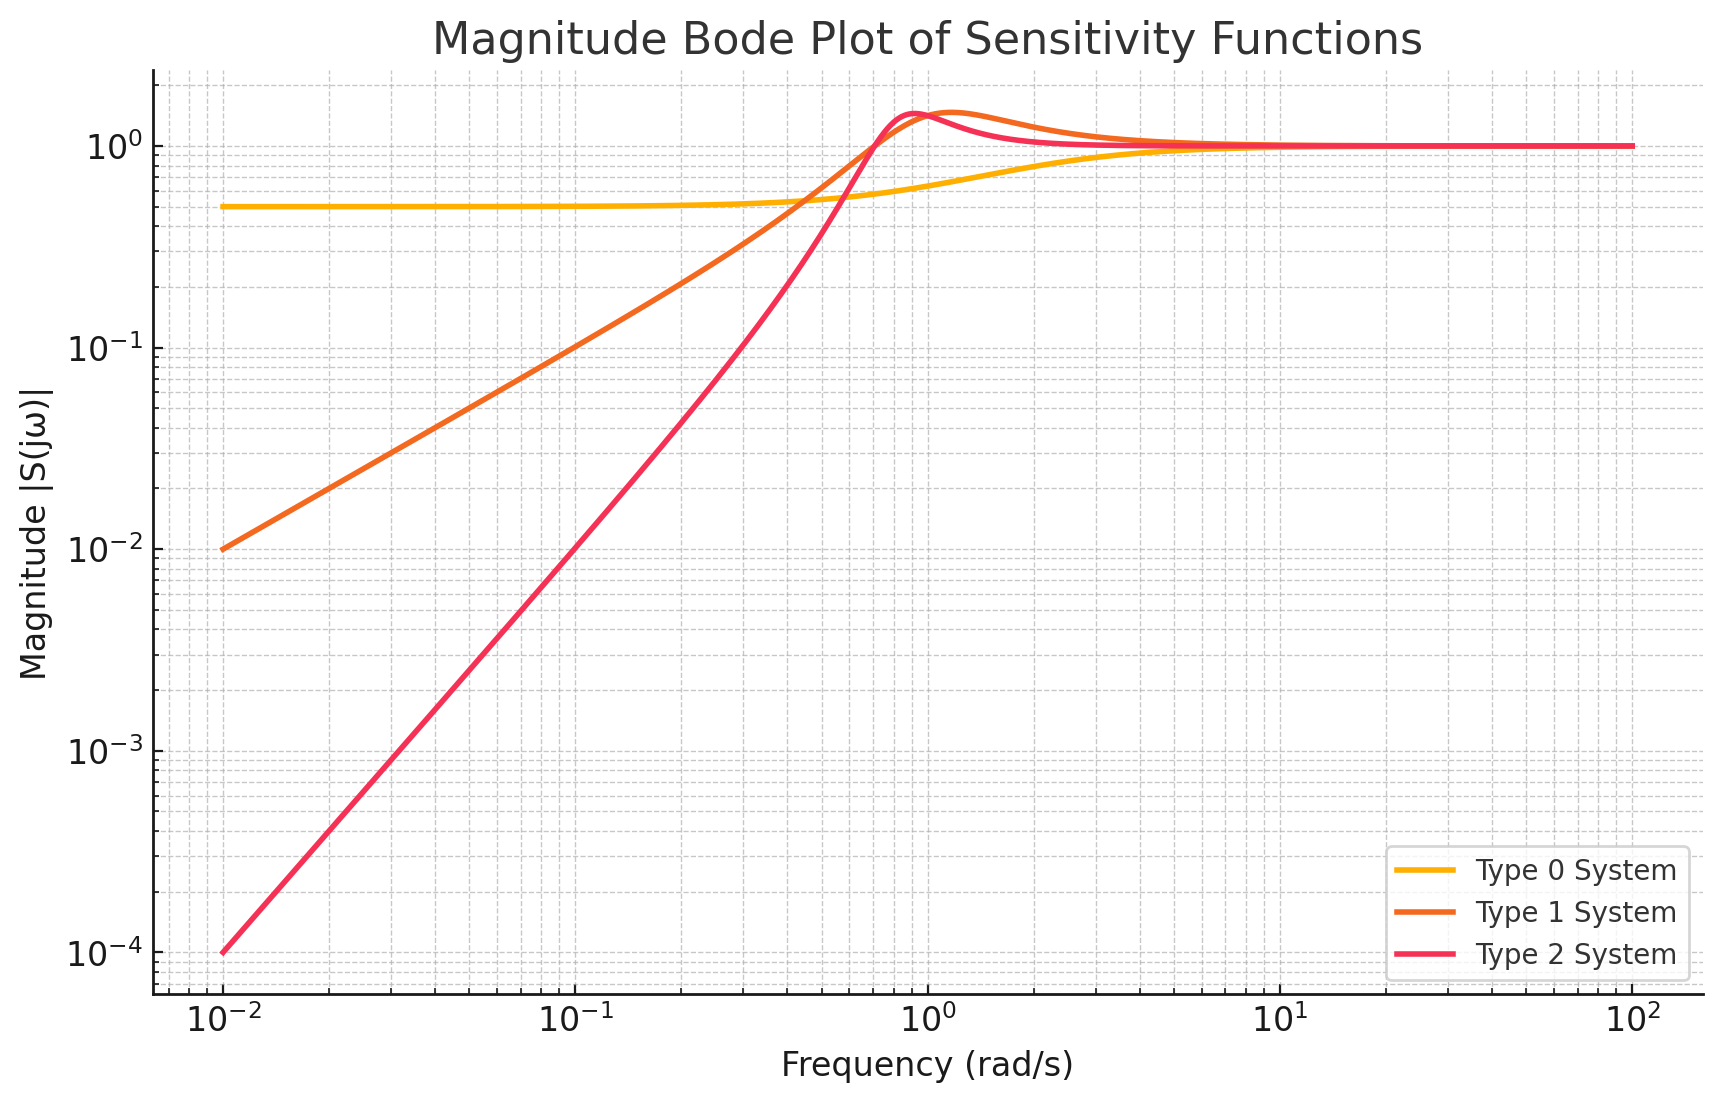
\includegraphics[width=0.75\textwidth]{sensitivity.png}
    \caption{The sensitivity function of 3 systems, the system type of which is indicated in the legend}
    \label{fig:sensitivity}
\end{figure}
One can realize that the sensitivity function of the second-order prototype has one zero at the origine, and therefore of system-type 1, but it is used for having a guidline studying transient requirements.
\[
S(s) = \frac{s(s+2\zeta\omega_n)}{s^2 + 2\zeta\omega_ns + \omega_n^2}
\]
\end{QandAbox}

A general sensitivity function $S(s)$, is considered as the follwoing form:\[
S(s) = s^{\nu + p}S^{*}(s)
\]
\newpage
\section{Steady-state resopnse to polynomial reference inputs}
For this class of specifications, the following form of constraint can be derived for $S^{*}(s)$.

\begin{figure}[H]
    \centering
    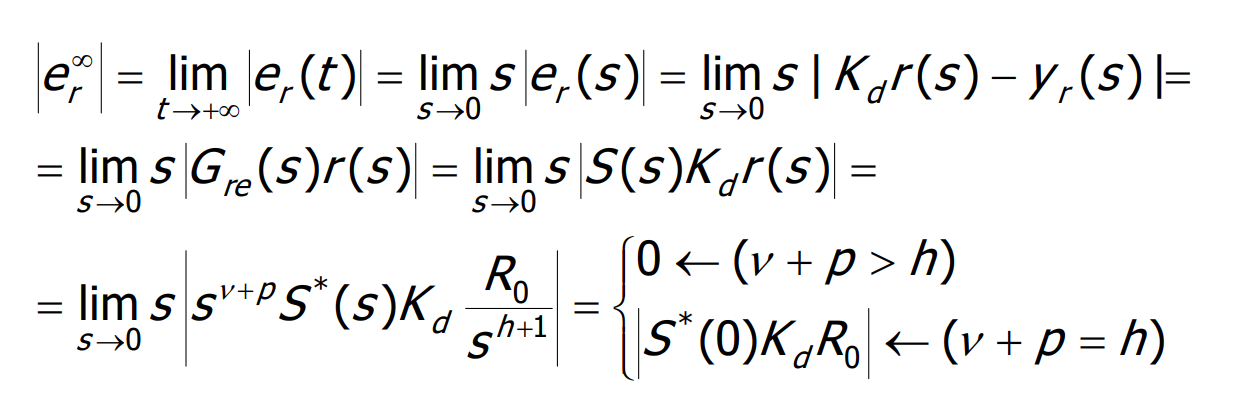
\includegraphics[width=0.5\textwidth]{ss-input.png}
    \caption{Constraint on the sensitivity function as a consequence of a specification on the steady-state input error at the presence of a polynomial input signal.}
    \label{fig:ss-input}
\end{figure}

In the case, $\rho_r = 0$ no constraint on the norm of $S^{*}$ is obtained. Also in the previous approach, if steady-state output error was required to be zero, no constriant on $K_c$ would be obtained.
\begin{factbox}[Some Reminders]
Having the frequency response of a function in the form of:
\[
H(s) = \frac{k_\nu}{s}\frac{(1 + \frac{s}{1})}{1 + \frac{s}{10}}
\]
the generalized dc-gain can be obtained in the following manner.
\begin{figure}[H]
    \centering
    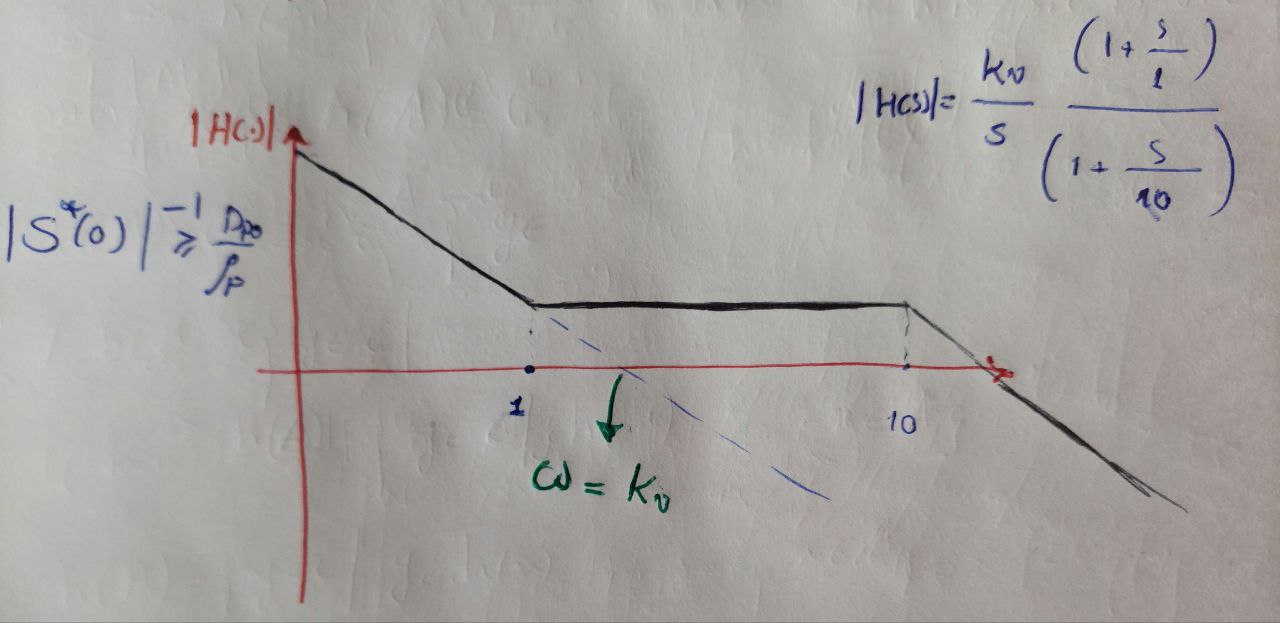
\includegraphics[width=0.75\textwidth]{dc-gain-s-1.jpg}
    \caption{}
    \label{fig:}
\end{figure}

Now, for the case that $H(s)$ has the same structure as sensitivity function.

\begin{figure}[H]
    \centering
    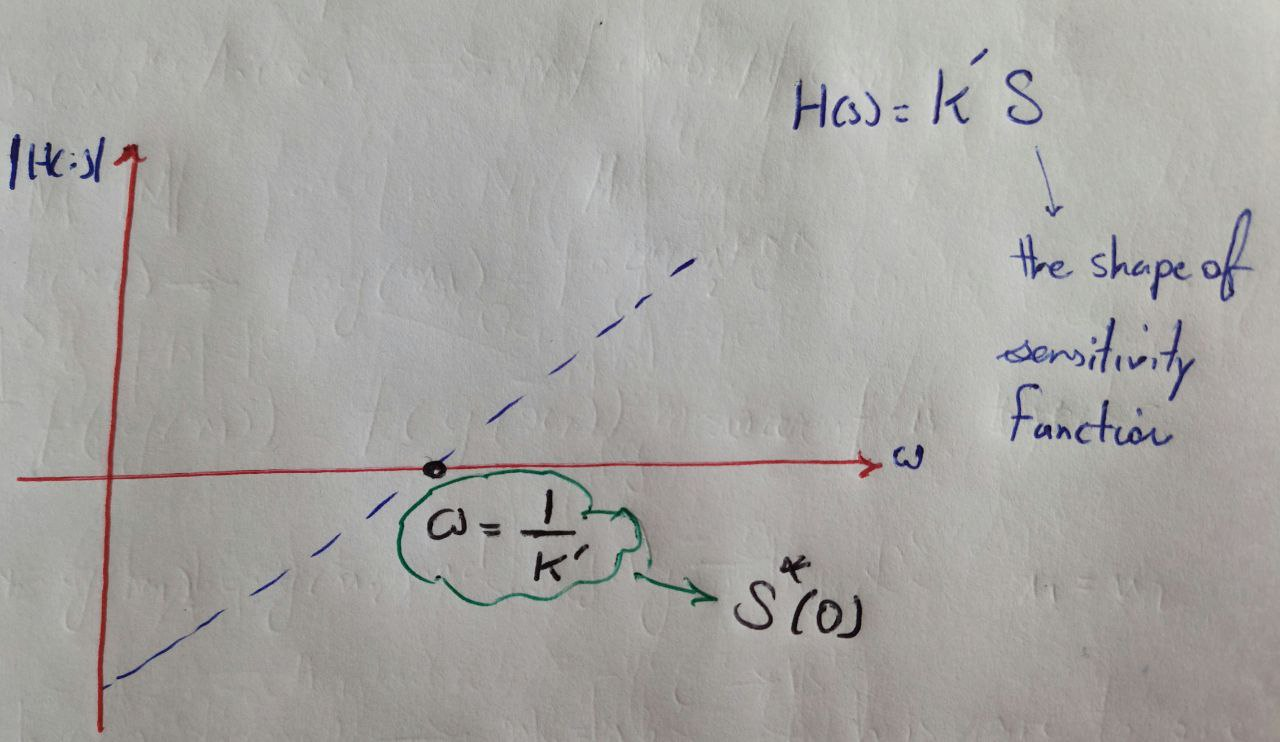
\includegraphics[width=0.75\textwidth]{dc-gain-s.jpg}
    \caption{}
    \label{fig:}
\end{figure}

\end{factbox}

\begin{factbox}[S-plane of the poles of a 2nd-order prototype system]
\begin{figure}[H]
    \centering
    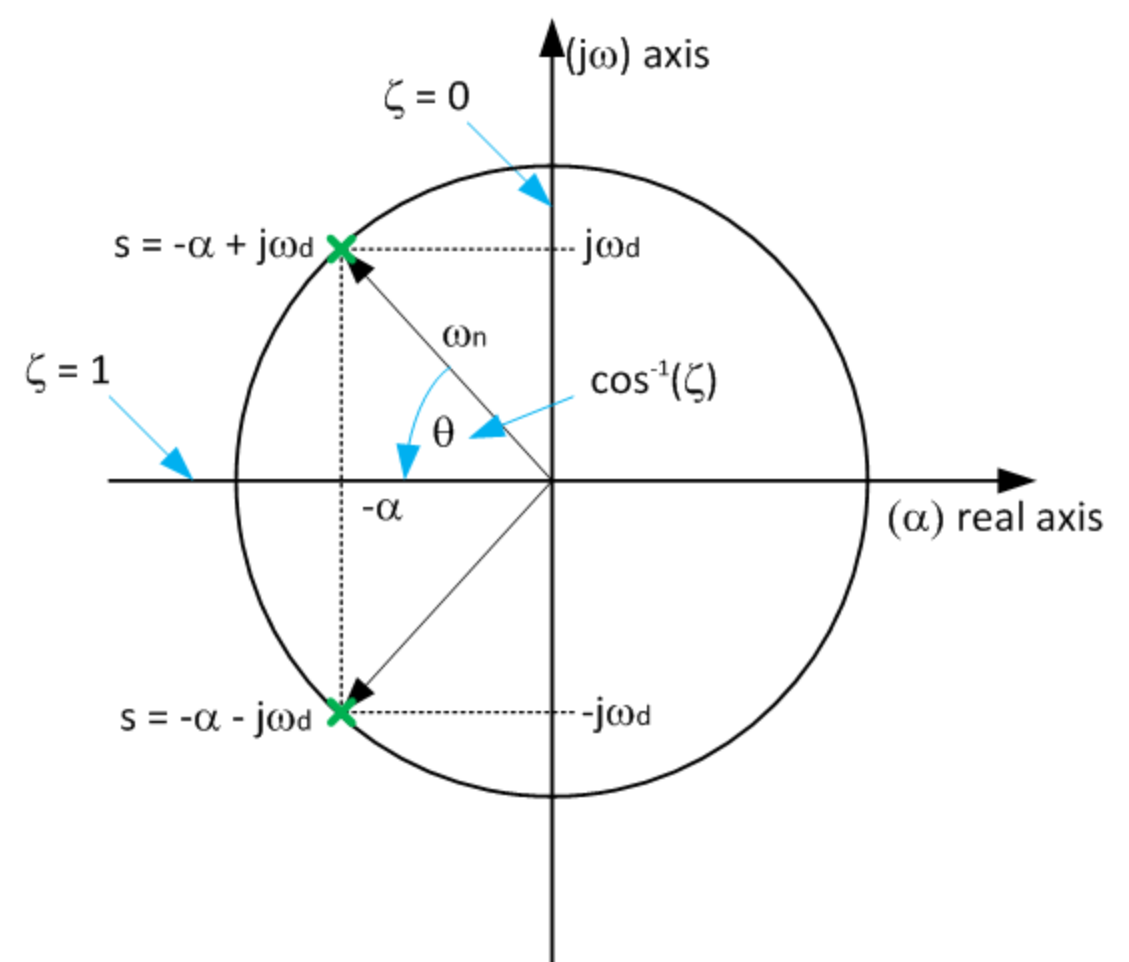
\includegraphics[width=0.5\textwidth]{s-plane.png}
    \caption{}
    \label{fig:}
\end{figure}
\end{factbox}

\section{Rational approximation of frequency constraints}
Rational functions of the variable $s$ are used to approximate the frequency domain constraints on $S$ and $T$. The parameters of the approximating fucntions(steady-state gain, zeros, and poles) can be moved to get the desired result. \textbf{Butterworth polynomials} can be used either as denominator or numerator of the approximating rational function to effectively retain constraints on different frequency ranges.

\subsection{Butterworth polynomials}

\begin{figure}[H]
    \centering
    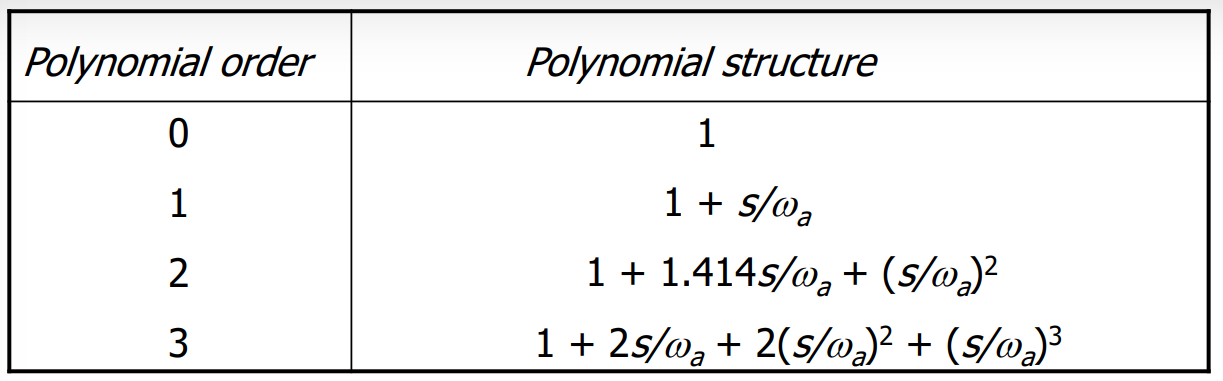
\includegraphics[width=0.75\textwidth]{butterworth.png}
    \caption{table of butterworth polynomials}
    \label{fig:butterworth}
\end{figure}

When a Butterworth polynomial is used as numerator (denominator) of a rational function, the magnitude of the frequency response at frequency $\omega_a$ is increased (decreased) by +3dB (-3dB) irrespective of the order of the polynomial.

Butterworth polynomials are used to obtain a rational function $W^{-1}_S(s)$ in such a way that $|W^{-1}_S(j\omega)|$ satisfies the constraints regarding $S(s)$.
\[
|W_S^{-1}| \leq M_S^{LF} \:\:\:\forall \omega_p \leq \omega_p⁺,\,\,\, \max\limits_{\omega}|W_S^{-1}(\infty)|\leq S_{p0}
\]
Butterworth polynomials are used to obtain a rational function $W_T^{-1}(s)$ in such a way that $|W^{-1}_T(j\omega)|$ satisfies:

\[
|W_T^{-1}| \leq M_T^{HF} \:\:\:\forall \omega_s \geq \omega_s^-,\,\,\, \max\limits_{\omega}|W_T^{-1}(\infty)|\geq T_{p0}
\]

$W_T^{-1}$ is required to satisfy:
\[
|W_T^{-1}| \leq M_S^{HF} \:\:\:\forall \omega_s \leq \omega_s⁻,\,\,\, |W_T^{-1}(0)|= T_{p0}
\]


\section{Performance specification as $H_{\infty}$ norm constraints}
Let us call:
\begin{itemize}
\item $W_S(s)$ the inverse of the rational approximation of the frequnecy domain constraints on the functiono $S(s)$
\item $W_T(s)$ the inverse of the rational approximation of the frequency domain constraints on the funtion $T(S)$
\end{itemize}

Design constraints obtained from the considered preformance requirements can be written in the following compact form:
\[
|T(j\omega)|\leq |W_T^{-1}|\,,\, |S(j\omega)| \leq |W_S^{-1}(j\omega)| \:\forall \omega
\]
or equivalently:
\[
|W_T(j\omega)T(j\omega) \leq \ \,,\, |W_S(j\omega)S(j\omega)|\leq \:\forall \omega
\]
Now, let us define the $H_{\infty}$ norm of a SISO LTI system with transfer function $H(s)$ as:
\[
\|H(s)\| := \max\limits_{\omega}|H(jw)|
\]
By exploring this definition, we can rewrite the design constraints obtained from the considered performance requirements in terms of the weighted $H_\infty$ norm of $S(s)$ and $T(s)$:
\[
\|W_T(s)T(s)\|_\infty \leq 1 \,,\, \|W_s(s)S(s)\|_\infty \leq \
\]

\begin{factbox}[information regarding the bode diagram of zeros and poles at 0]
example:
\(
H_1(s) = k_v \frac{H_1^*(s)}{s}
\),
here $v$ historically refer to velocity.
\end{factbox}

\section{Practicing shaping the weighting functions for sensitivity and complementary sensitivity function}
\begin{factbox}
Here, it is shown that how the frequency at which the asymptote of a transfer function passes the 0 dB axis is related to the DC gain of the transfer function.
\begin{figure}[H]
    \centering
    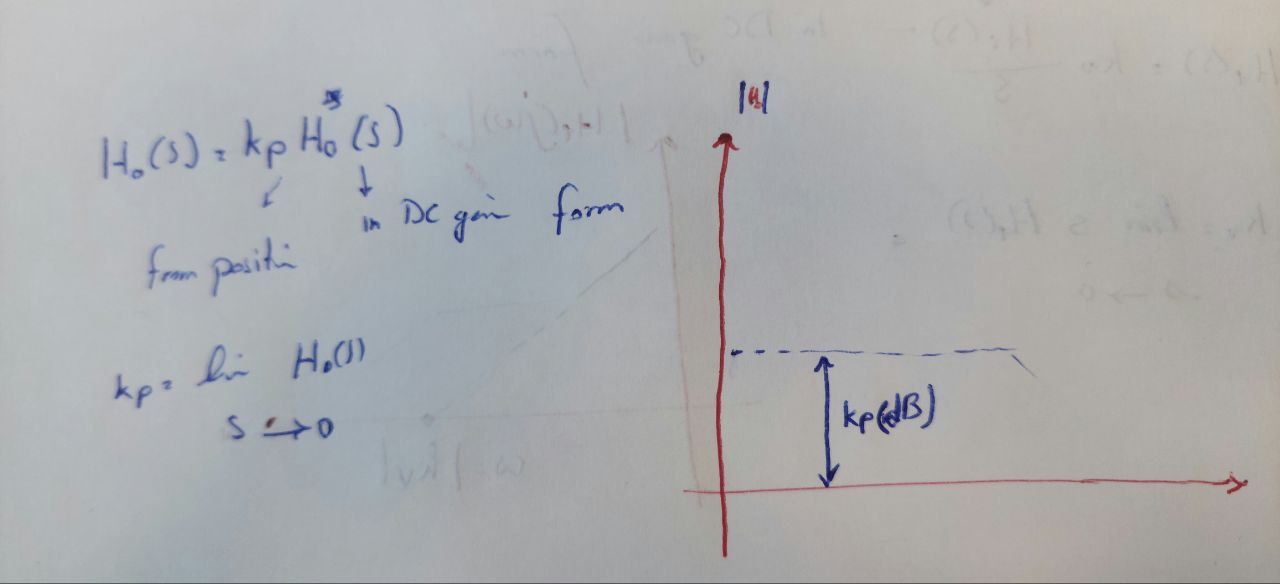
\includegraphics[width=0.75\textwidth]{H0.jpg}
    \caption{example 01}
\end{figure}
\begin{figure}[H]
    \centering
    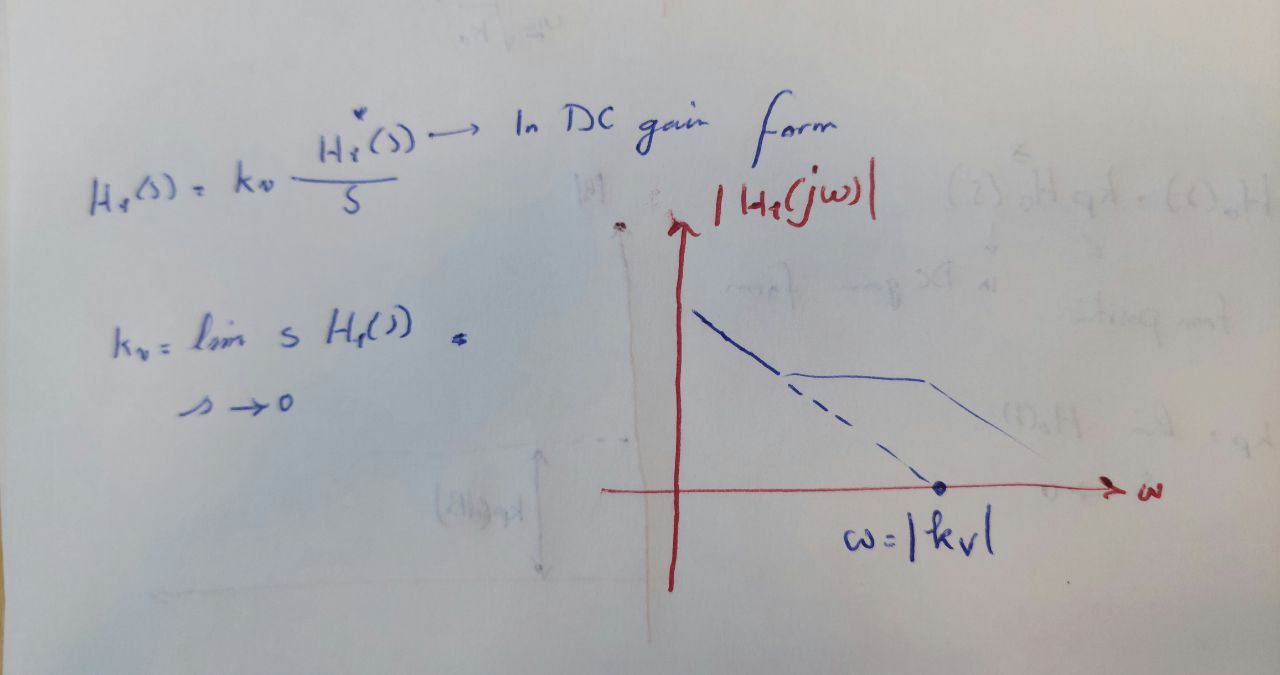
\includegraphics[width=0.75\textwidth]{H1.jpg}
    \caption{example 02}
\end{figure}
\end{factbox}

\begin{factbox}
\begin{figure}[H]
    \centering
    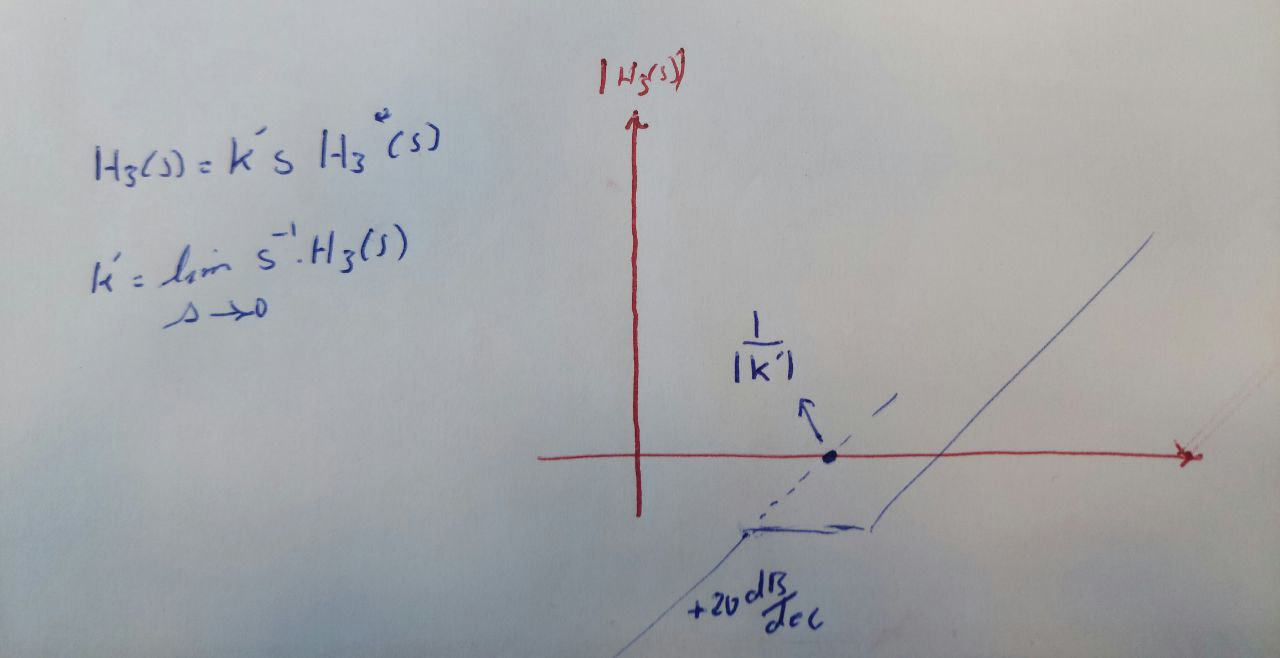
\includegraphics[width=0.75\textwidth]{H3.jpg}
    \caption{example 03}
\end{figure}
\begin{figure}[H]
    \centering
    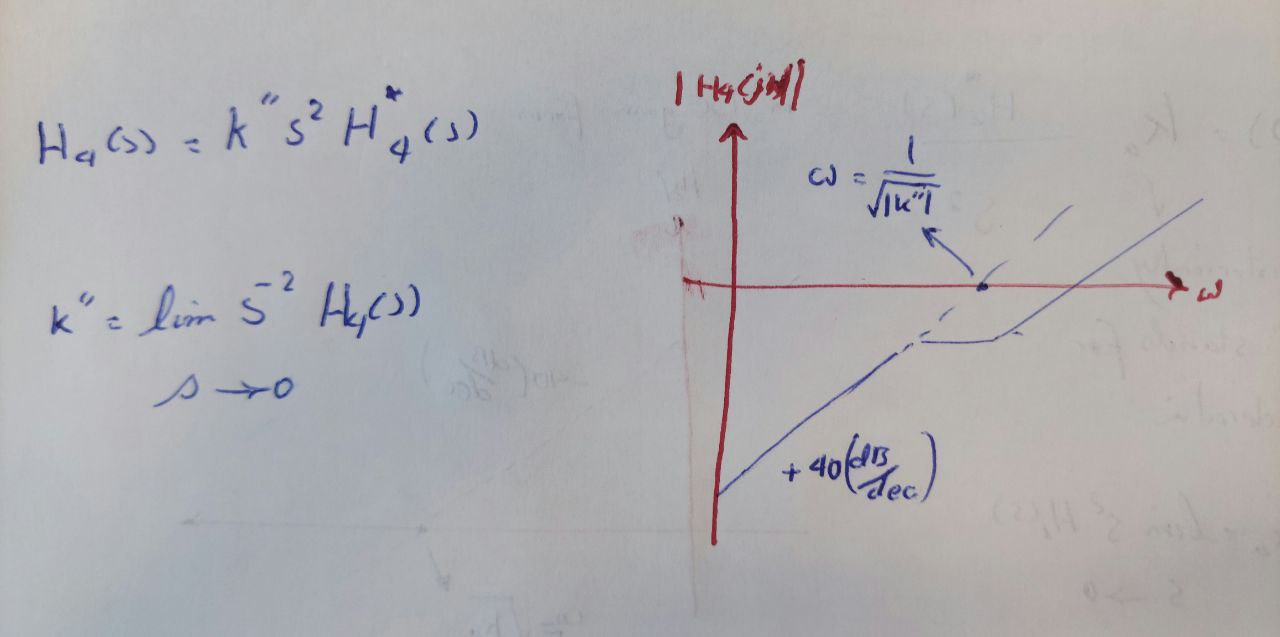
\includegraphics[width=0.75\textwidth]{H4.jpg}
    \caption{example 04}
\end{figure}
\end{factbox}

\section{shaiping the weight functions for S and T}
These weighting functions are going to be used in order to use the optimizer to obtain a controller in the $H_\infty$ method, as well as checking the robust stability and performance of the system final.


Just bear in mind that the weighting functions obtained in this stage are not exact, since we are using second-order prototype system for translating the requirements on the transient, and since we just use fractional transfer functions in order to shape the weight functions. \textbf{requirements on the steady-state performance are exact thanks to the fact that it depends on the known parameters like the system type of the system and disturbance assumptions.}

\subsection{Shaping $W_S$, the weighting function on the sensitivity funciton}
Consider the following constraints for our sensitivity function:
\[
M_S^{HF} = -60 \:dB \:\:\: \forall \:\omega \in (-\infty, \omega_p^{+}=1]
\]
\[
\zeta = 10 \:\% \: \Rightarrow \:\: S_{p_0} = 1.36
\]

The following weighting function can be considered as our first attempt:
\[
W_S^{-1} = k \frac{1 + \frac{s}{z_1}}{1 + \frac{s}{p_1}}
\]
where $ k = 0.001$ is equivalent to -60 $dB$. we put a zero at 1 in order to increase the magnitude, and \textbf{we compute the following limit in order to put our pole in a position to reach $S_{p0}$ when the frequency tends to infinity;} the reasult is a pole at $\omega = 1360 rad.sec^{-1}$.
\[
\lim\limits_{s \to \infty} W_S^{-1} = k \frac{p_1}{z_1} = S_{po} \Rightarrow p_1 = \frac{S_{p0}z_1}{k} = 1360
\]

\begin{figure}[H]
    \centering
    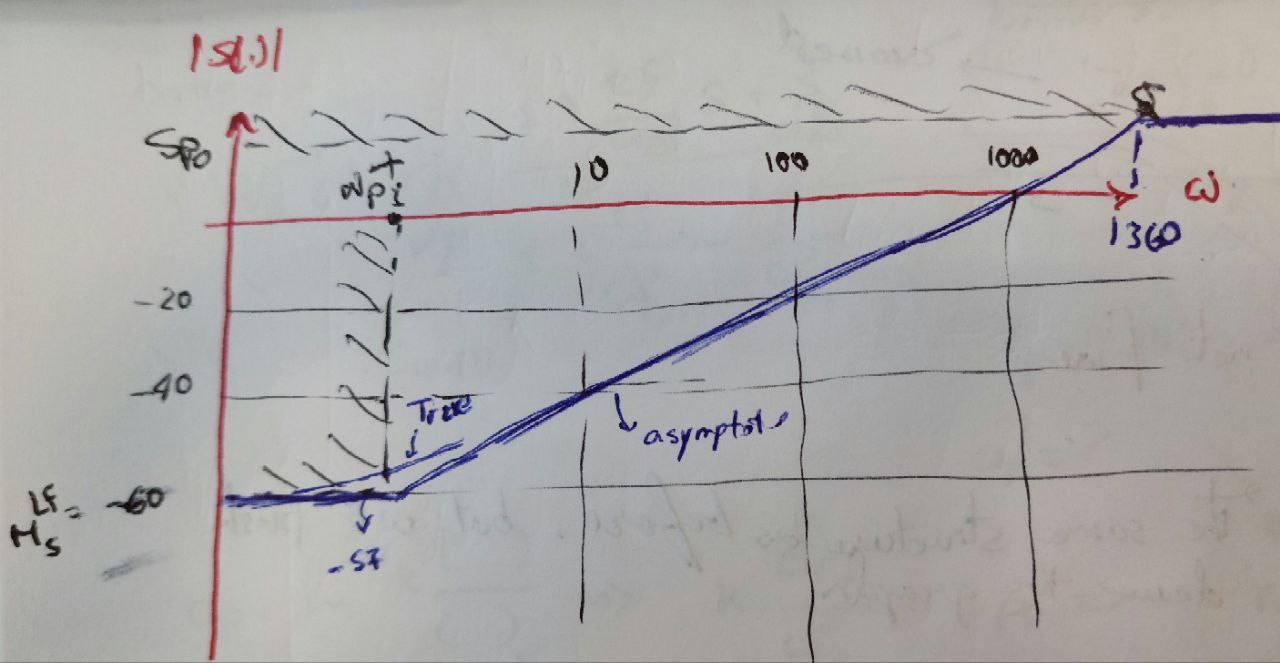
\includegraphics[width=0.75\textwidth]{ws-first.jpg}
    \caption{The first attempt to shape the weighting function}
\end{figure}

This solution is not fine, since based on the real behavior of the Bode of this transfer function, at $\omega = 1$, the magnitude increases by +3 $dB$, which is because of the first-order zero at $\omega = 1$, thereby passing the forbidden region; in other words, the requirement on the low frequency performance is not going to be satisfied. Another problem is that, having such a high crossover frequency and also taking into consideration the complementary sensitivity function, in this case $1000 Hz$, we may obtained infeasibility when optimizing for the controller.  \\

In the second attempt, one may decreases the value of dc-gain to $-63 dB$ in order to circumvent the first problem. However, doing so, the result of the limit which leads to the frequency of the pole leads to the frequency $1924$, making the situation even worst for the second issue.
\begin{figure}[H]
    \centering
    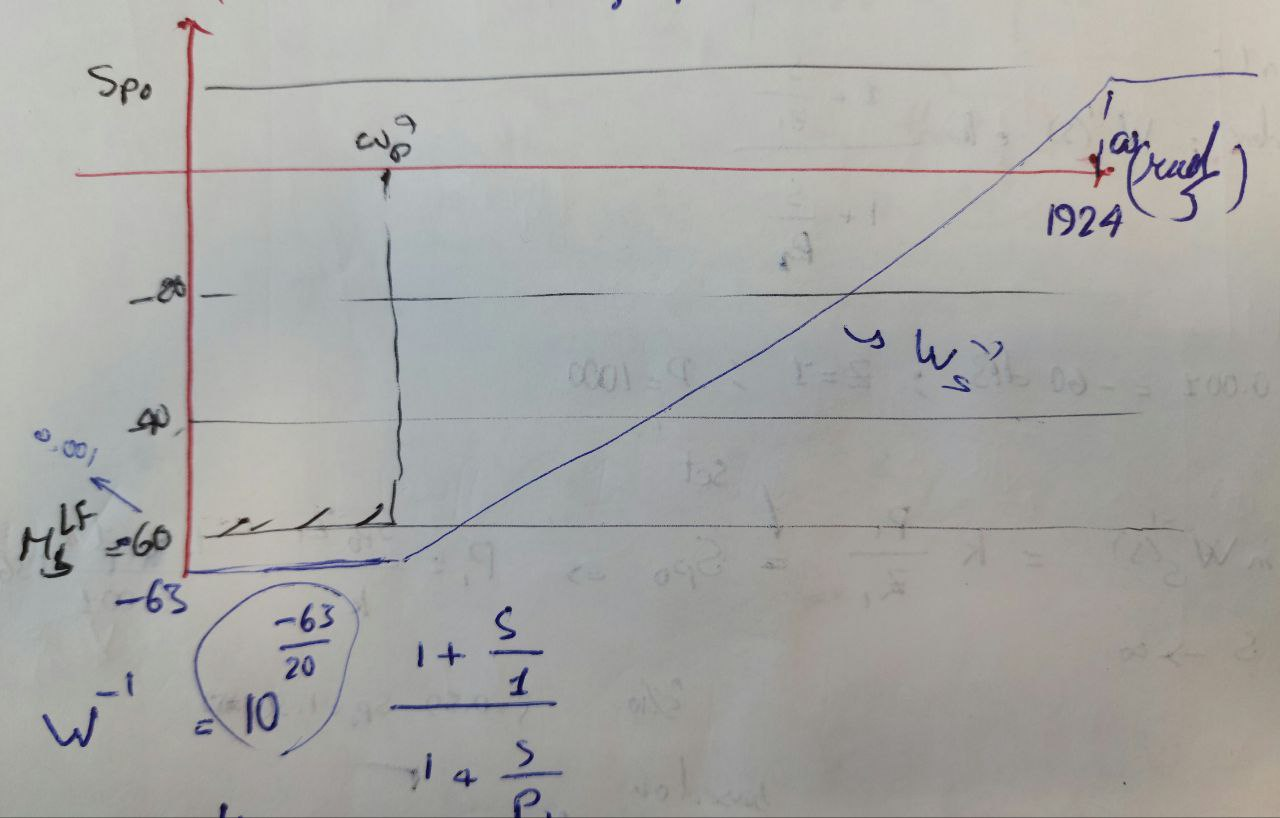
\includegraphics[width=0.75\textwidth]{ws-second.jpg}
    \caption{The second attempt to shape the weighting function}
\end{figure}


A third attempt might be using a butterworth polynomial in the both nominator and denominator of the weighting function. In this case, the both problems are tend to be solve, yet there is the chance that \textbf{the crossover frequency of $S$ become lower than requirements -  resulting in a slow transient performance due to the low crossover frequency.}\\

Considering the first problem of the homework, the system type of the loop function should be 1 so that the final system guarantees the steady-state performance requirements. \textbf{As the sensitivity function has the same number of zeros at 0 as the system type of the system.} so we start with the following inverse weighting function
\[
W_S^{-1} = s^{\nu + p} S^{*}(0) = 0.15s
\]
\textbf{consider that 0.15 determines some of the steady-state requirement performance for the sensitivity function, and the final dcgain of the sensitivity function should be less than this value. Leading to a higher $K_c$ in the loop shaping context.}

and then, we try to stay as close as possible to the prototype-second order system, due to the fact that the optimizer has a higher chance in order to find a solution that is as close as possible to a second order system. Finally, the limit should be used in order to make sure that when the frequency tends to infinity, the value of the inverse weighting function tends to $S_{p0}$. \\

The order of the zeros and poles to add to this first structure is as follows in the first attempt:
\begin{itemize}
    \item one zero to get close the second order prototype system.
    \item then, we need two poles in order to reduce the +40 slop to 0. when adding these poles, ideally we are willing to get as close as possible to the knee of the second-order sensitivity function.
\end{itemize}

The result is going to be like the follwoing figure.

\begin{figure}[H]
    \centering
    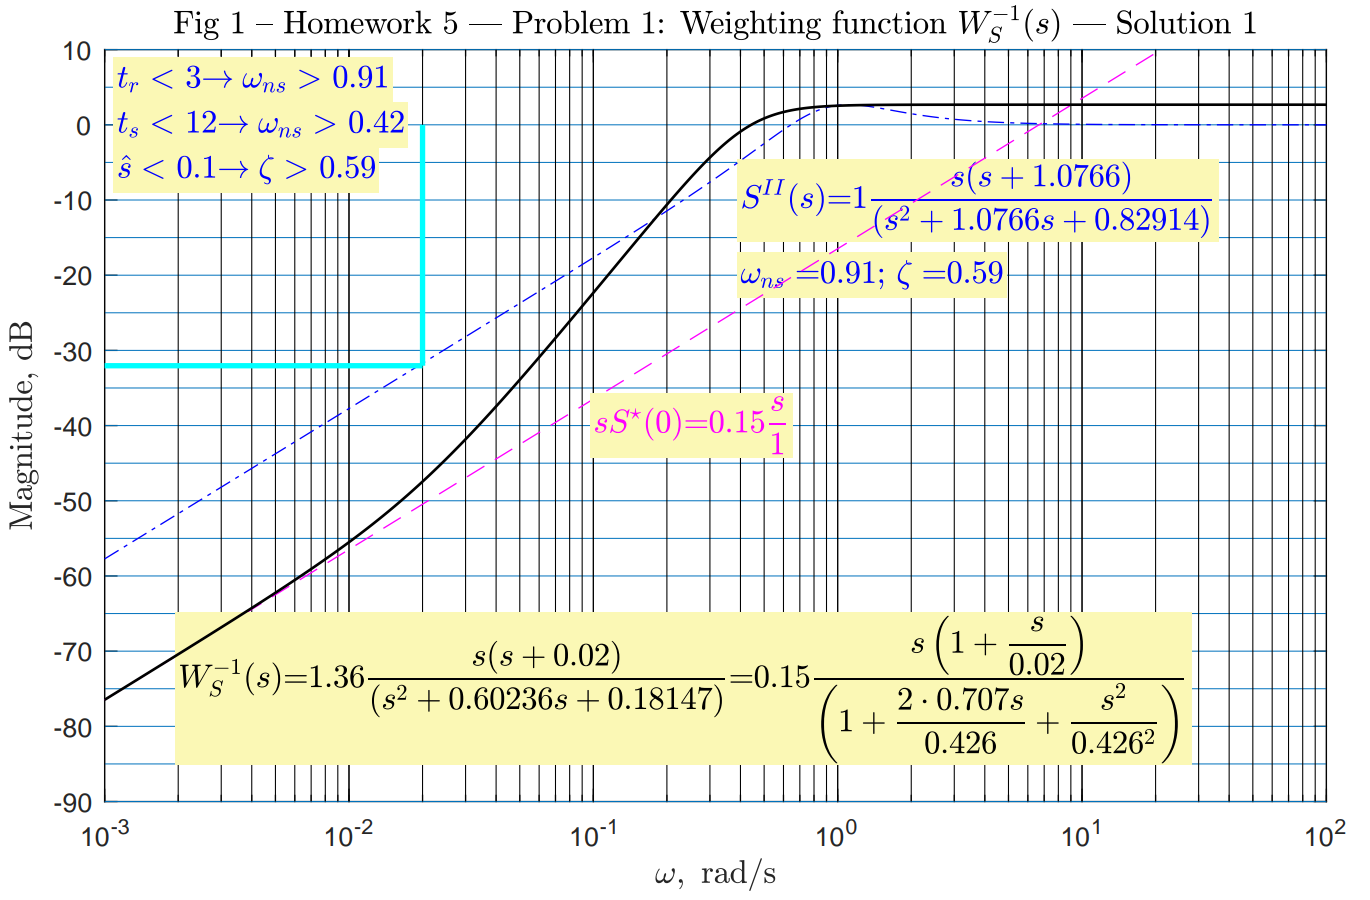
\includegraphics[width=0.75\textwidth]{h1-ws-first.png}
    \caption{The first attempt for $W_S^{-1}$ for the first problem of the homework.}
\end{figure}

As it can be seen, this weighting function may result in a slow system; As, in the contrary, if the crossover freequency is large than the one of thte second-order system, the resulting system is going to be faster than needed, or \textbf{bandwidth demanding}.

To resolve this issue, the position of the zero can be changed to a bit higher frequency in order to lead to the following result.

\begin{figure}[H]
    \centering
    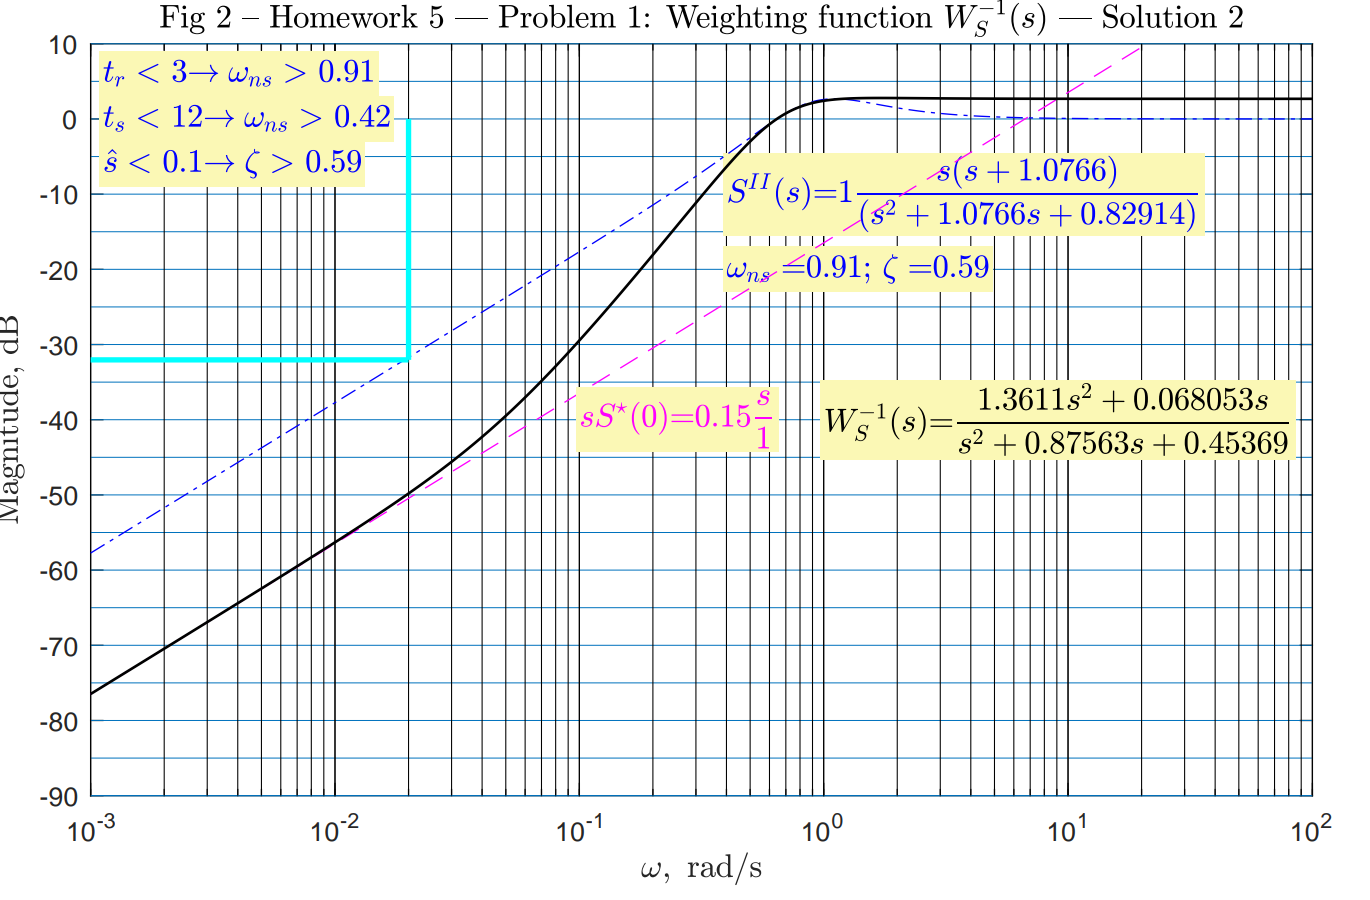
\includegraphics[width=0.75\textwidth]{h1-ws-second.png}
    \caption{The second attempt for $W_S^{-1}$ for the first problem of the homework.}
\end{figure}


To make the inverse weighting function to be tight as far as possible, the following weighting function can be used.

\begin{factbox}
According to the professor, the tightest the $W_S^{-1}$ to $S$, the simplest controller the optimizer is going to give.
\end{factbox}

A third attempt to make the weighting functino as tight as possible results in the following figure,

\begin{figure}[H]
    \centering
    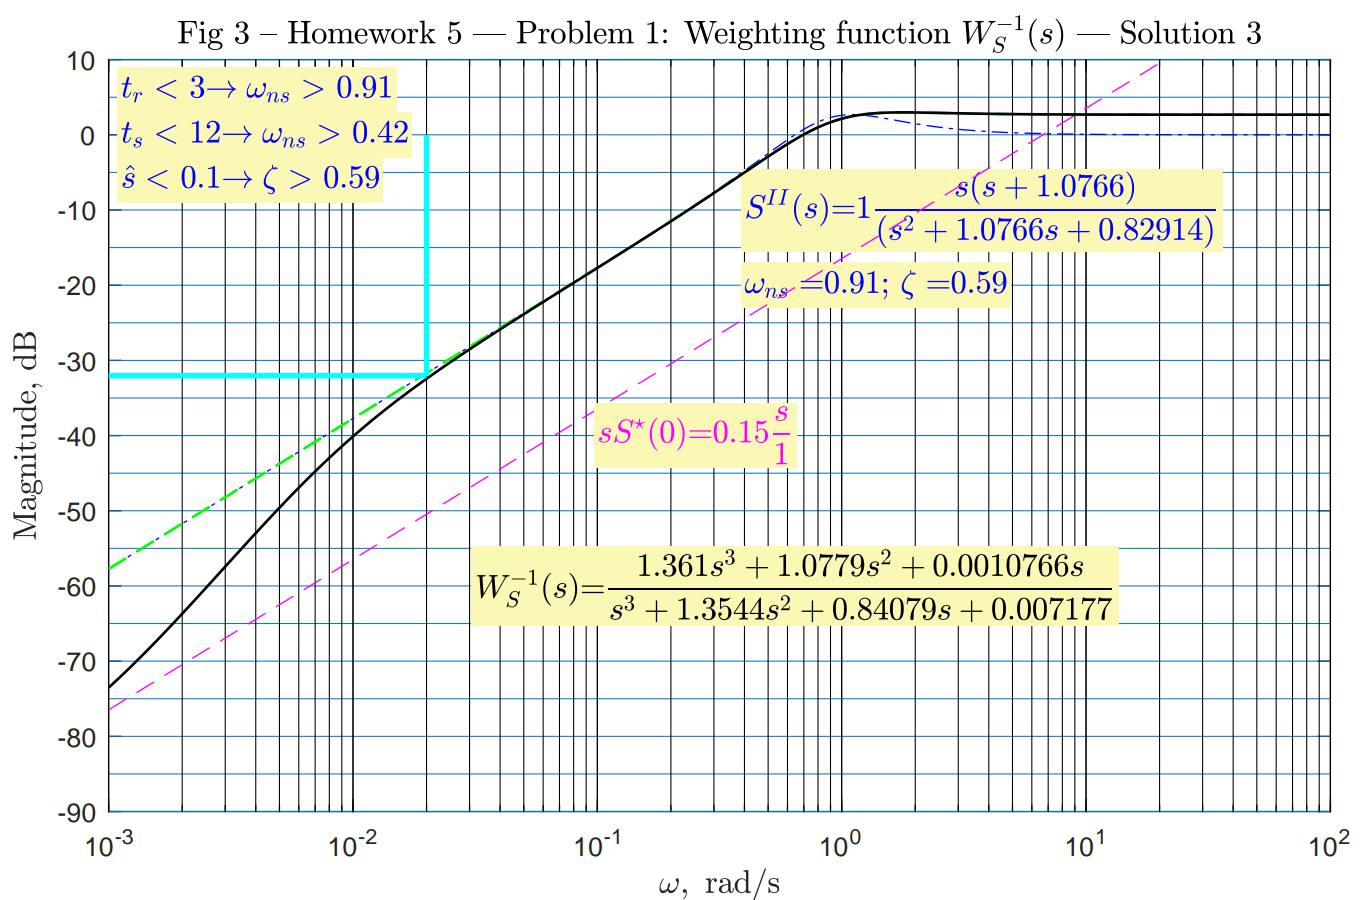
\includegraphics[width=0.75\textwidth]{h1-ws-third.png}
    \caption{The third attempt for $W_S^{-1}$ for the first problem of the homework.}
\end{figure}

In the end, $W_S$ is going to be simply the inverse of the $W_S^{-1}$

\subsection{Shaping $W_T$, the weighting function on the sensitivity funciton}
Here, it is much simpler. The procedure is as follows:
\begin{enumerate}
    \item We need to make sure that as $\omega$ tends to zero $W_T^{-1}$ is going to be at $T_{p0}$. Then, we start with
    \[
    W_T^{-1} = T_{p0}
    \]
    \item Then, we need to use a second-order butter worth function, and calculate the frequency of the poles so that the plot passes $M_T^{HF}$. The starting point is going to be as follows:
    \[
    T_{p0} - W_T^{-1}(\omega) = -40(\omega_p - \omega_s^{-})
    \]
    where
    $\omega_p$ is going to be used as the cutting frequency of the second-order butterworth function.
    
\end{enumerate}

